\section{UI Mockups}

The following section shows the mockup that where created to show the customer the 
layout of the iCare frontend, before the implementation was started.

\subsection{Dashboard}
\begin{figure}[H]
	\centering
	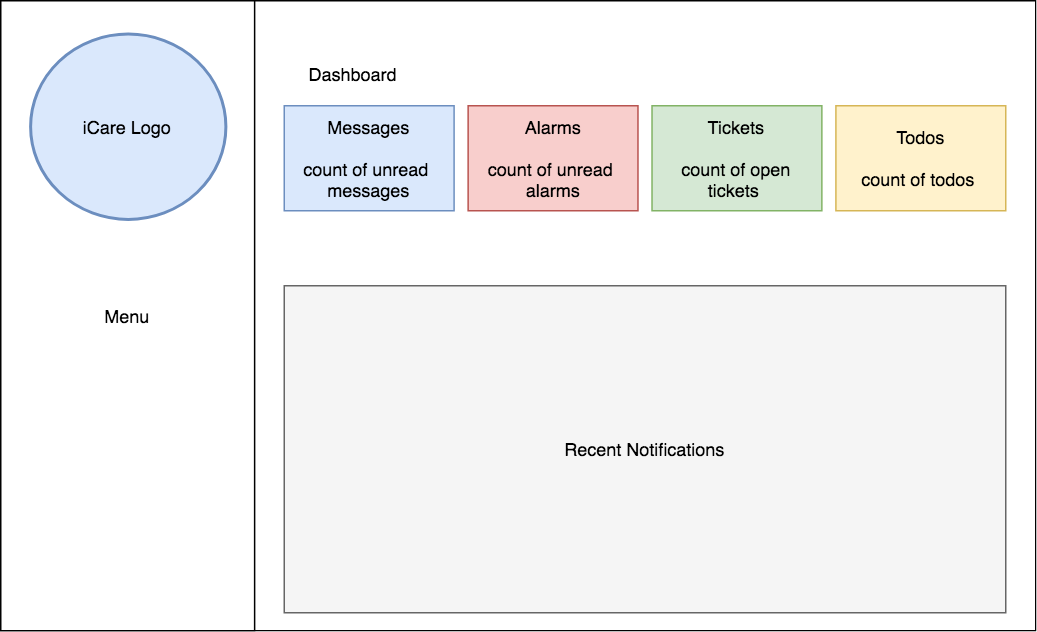
\includegraphics[width =0.65\textwidth]{images/mockDashboard.png}
	\caption{Mockup for dashboard page}
\end{figure}

\subsection{Tracking}
\begin{figure}[H]
	\centering
	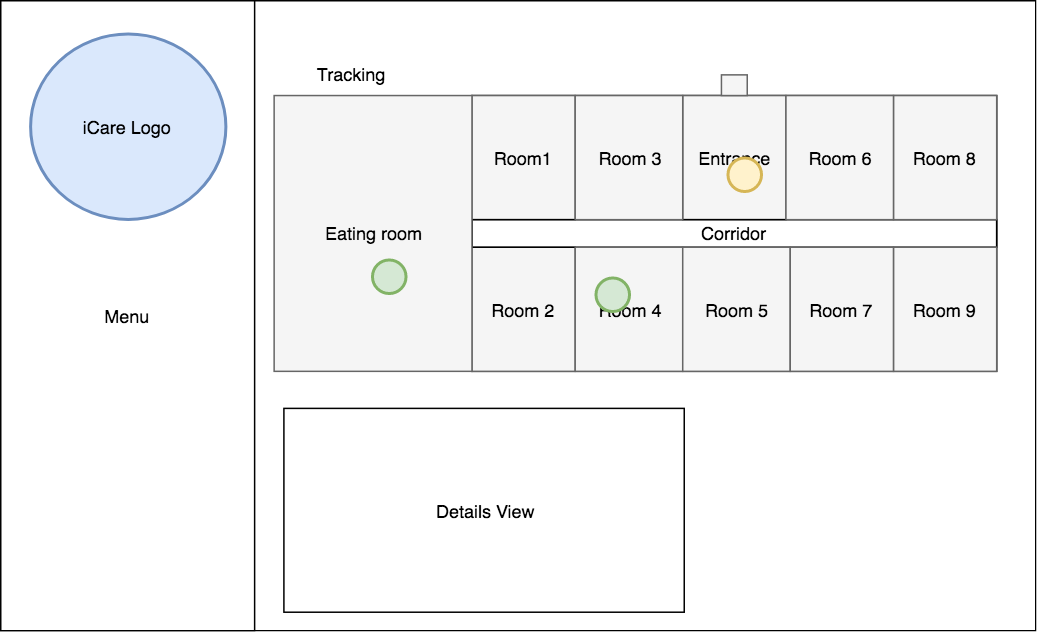
\includegraphics[width =0.65\textwidth]{images/mockTracking.png}
	\caption{Mockup for tracking page}
\end{figure}


\subsection{Eco Monitor}
\begin{figure}[H]
	\centering
	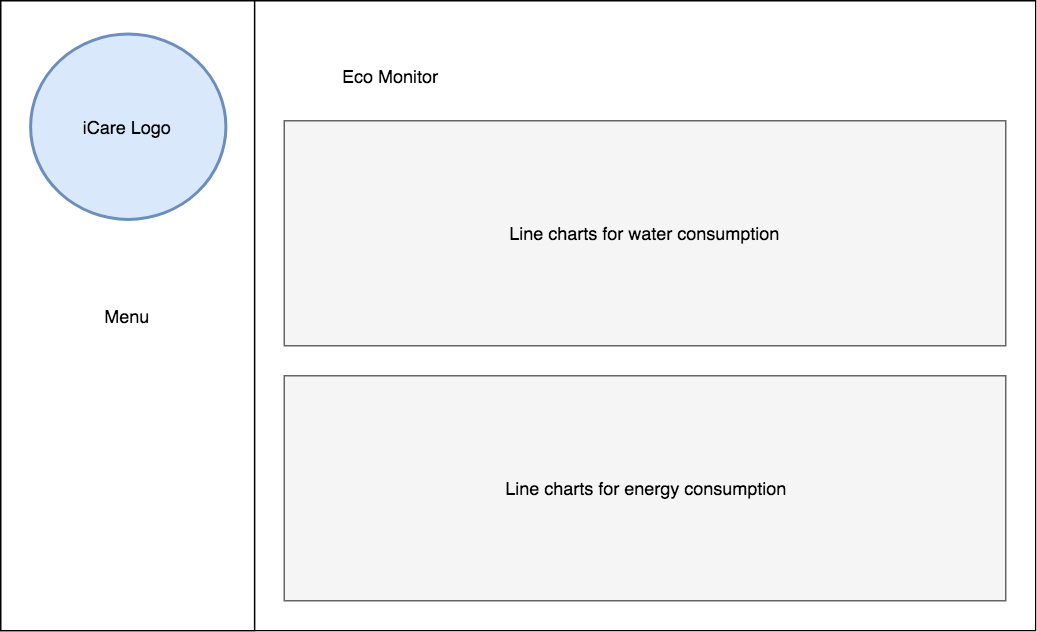
\includegraphics[width =0.65\textwidth]{images/mockEcoMonitor.png}
	\caption{Mockup for Eco Monitor page}
\end{figure}


\subsection{Cameras}
\begin{figure}[H]
	\centering
	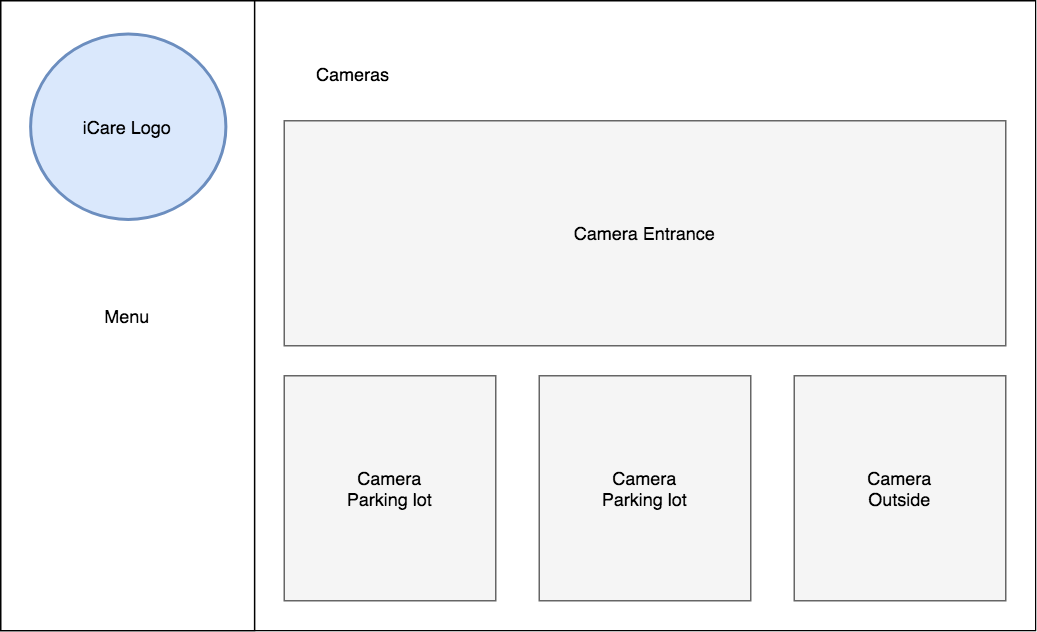
\includegraphics[width =0.65\textwidth]{images/mockCameras.png}
	\caption{Mockup for cameras page}
\end{figure}


\section{Implementation - Frontend}

The frontend was implemented with HTML, CSS and Javascript (ES6).
The following open source libraries were used:
\begin{itemize}

\item Chart.js to -  draw the diagrams in the Eco Monitor.
\item Date.js - to manipulate and format dates.
\item P5.js - to draw the interactive tracking interface.
\item Bootstrap 3 - a CSS framework to ensure a modern responsive user interface.
\end{itemize}


The focus in the design was placed on displaying the important messages (alarms) on each page so that staff can always see which new alarms have just been reported.
The user must manually mark these messages as read so that these messages are no longer displayed in the upper right-hand corner. For testing purposes during development, a Develop Tools page was implemented to manually force certain events to test the frontend end-to-end.

\subsection{Dynamic website}
Through timers the frontend calls the backend in the background at regular intervals (1 second), this ensures that the data in the frontend is always up-to-date.



\subsection{Dashboard / Notifications}

This page lists the latest notifications in the system in chronological order. 
At the top of the screen, the user also sees additional counters for the various categories: Messages, alerts, tickets and todos. If the user clicks on one of these four fields, a corresponding page appears, which displays the data in more detail.
It was important that an appropriate colour scheme was consistently followed.
Red means urgent information. Yellow, a warning that is not quite as urgent and green means information.
Each notification contains a time stamp, a message, a room in which the event occurred, and the inhabitant, if any.

\subsection{Notification popup}

When a specific event occurs, notifications are sent to the frontend. If the frontend receives a new message, it is stored in an inbox in the frontend. The number of unread notifications is displayed as a red box in the upper right corner of each page of iCare. As soon as at least one unread notification is in the inbox, this red box is displayed. This ensures that important messages do not appear only once and are then missed by the user.
Clicking on this popup takes the user to an overview page in which all unread notifications are listed. With one button, he can set all these messages to read. After that the inbox is empty and the red box is no longer displayed until a new notification arrives.
If notifications are removed from the inbox, they are not deleted, but are still displayed in the recent list in the dashboard.



\begin{figure}[H]
	\centering
	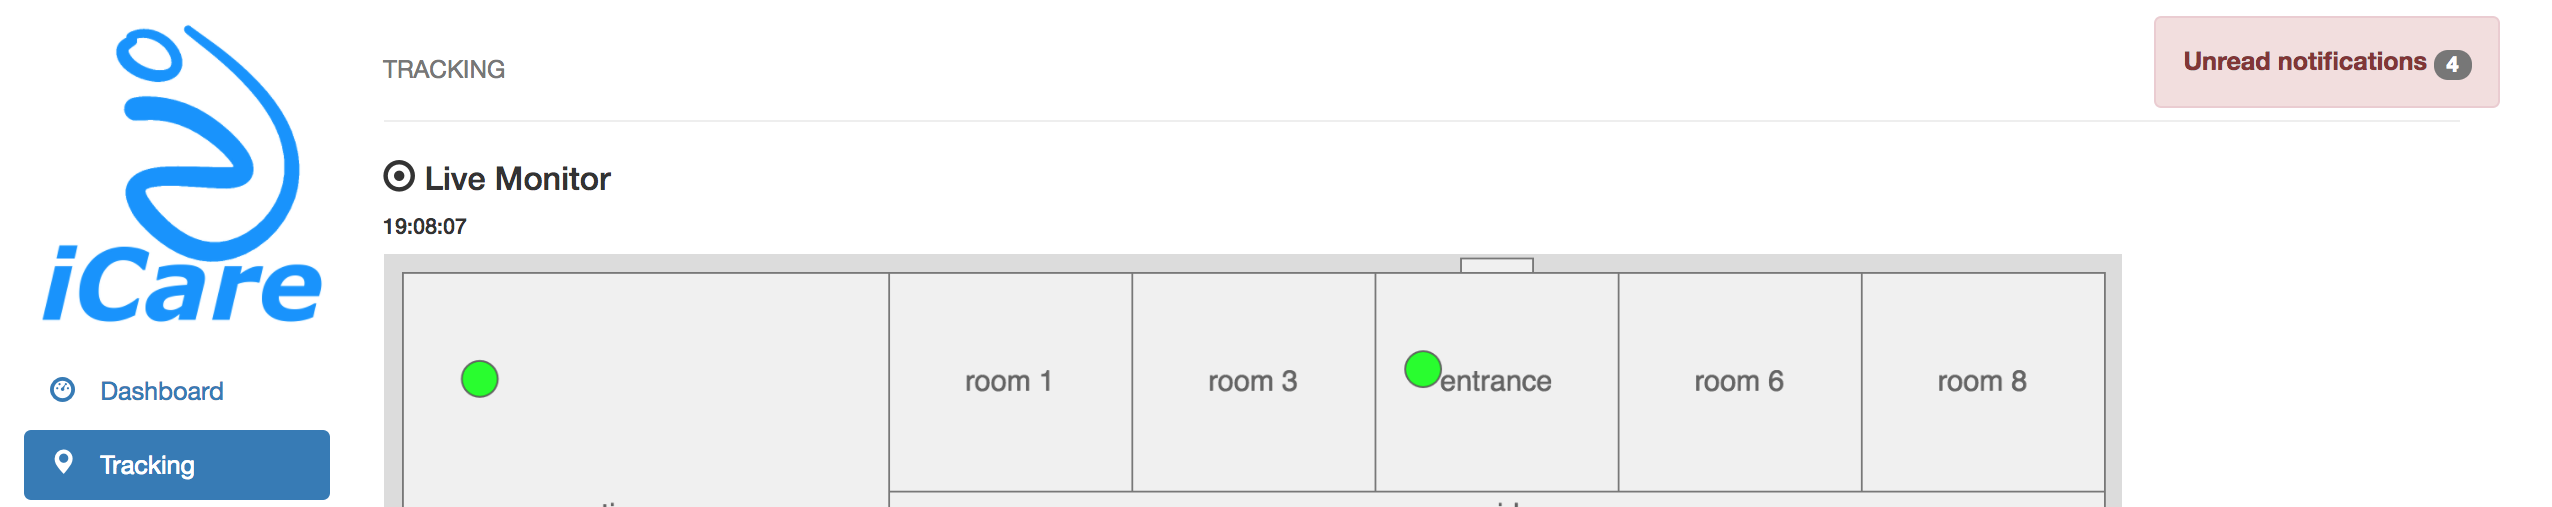
\includegraphics[width =1\textwidth]{images/uiNotificationPopup.png}
	\caption{UI screenshot Eco Monitor  page}
\end{figure}

\begin{figure}[H]
	\centering
	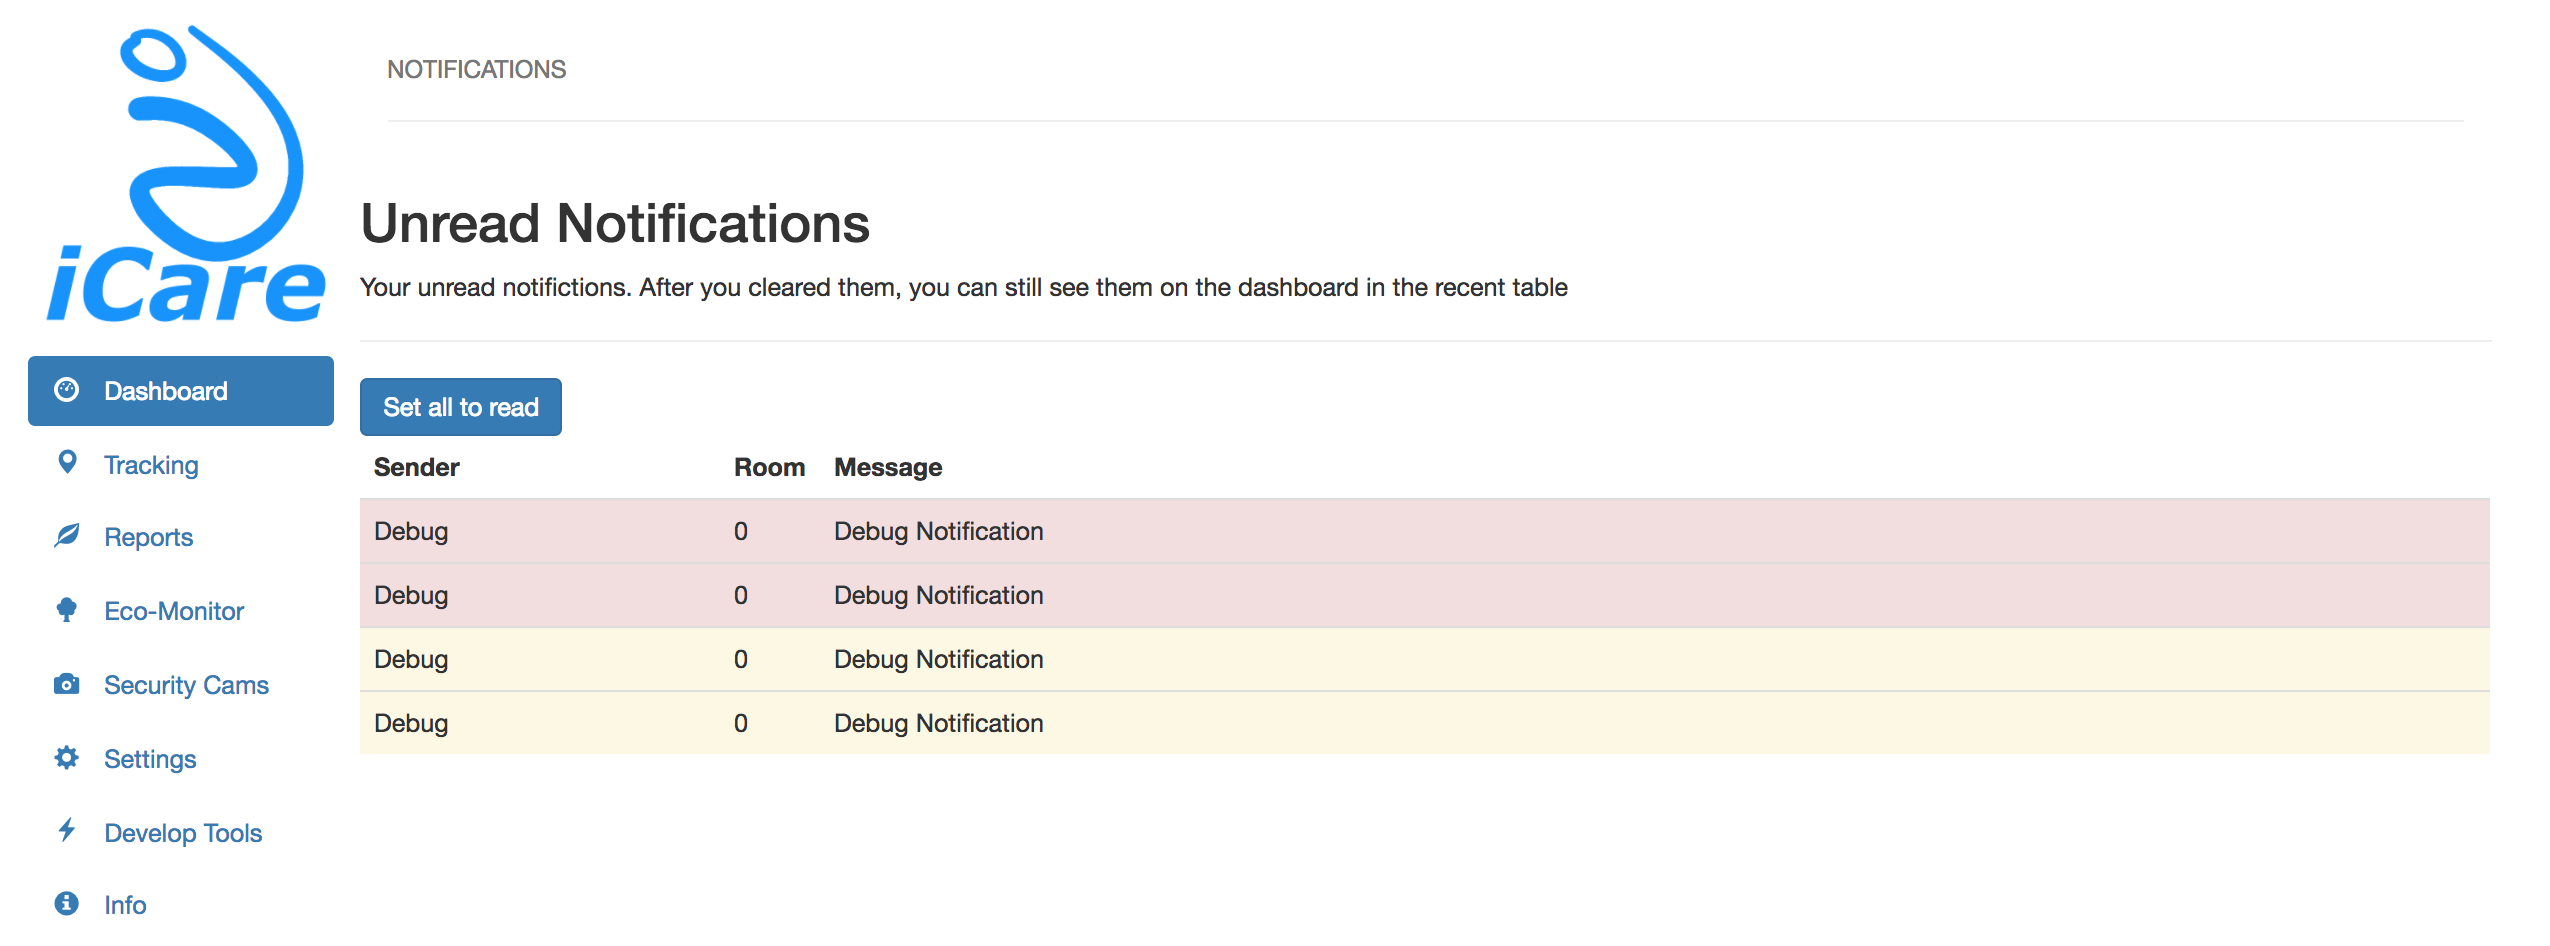
\includegraphics[width =1\textwidth]{images/uiUnreadNotifications.png}
	\caption{UI screenshot overview of unread notifications}
\end{figure}

\subsection{Tracking page}
On this page you can see a floor plan of the building showing the positions of the tracked inhabitants.
Every second the points are updated and the corresponding data is updated.
By clicking on a point, the current values of this inhabitant are displayed below the building floor plan ( Heart rate, Health Check, Restrictions, Name and ID).
The colors of the point have been implemented in a traffic light scheme. The dots on the floor plan, each representing an inhabitant, are displayed in these colors accordingly.


\begin{figure}[H]
	\centering
	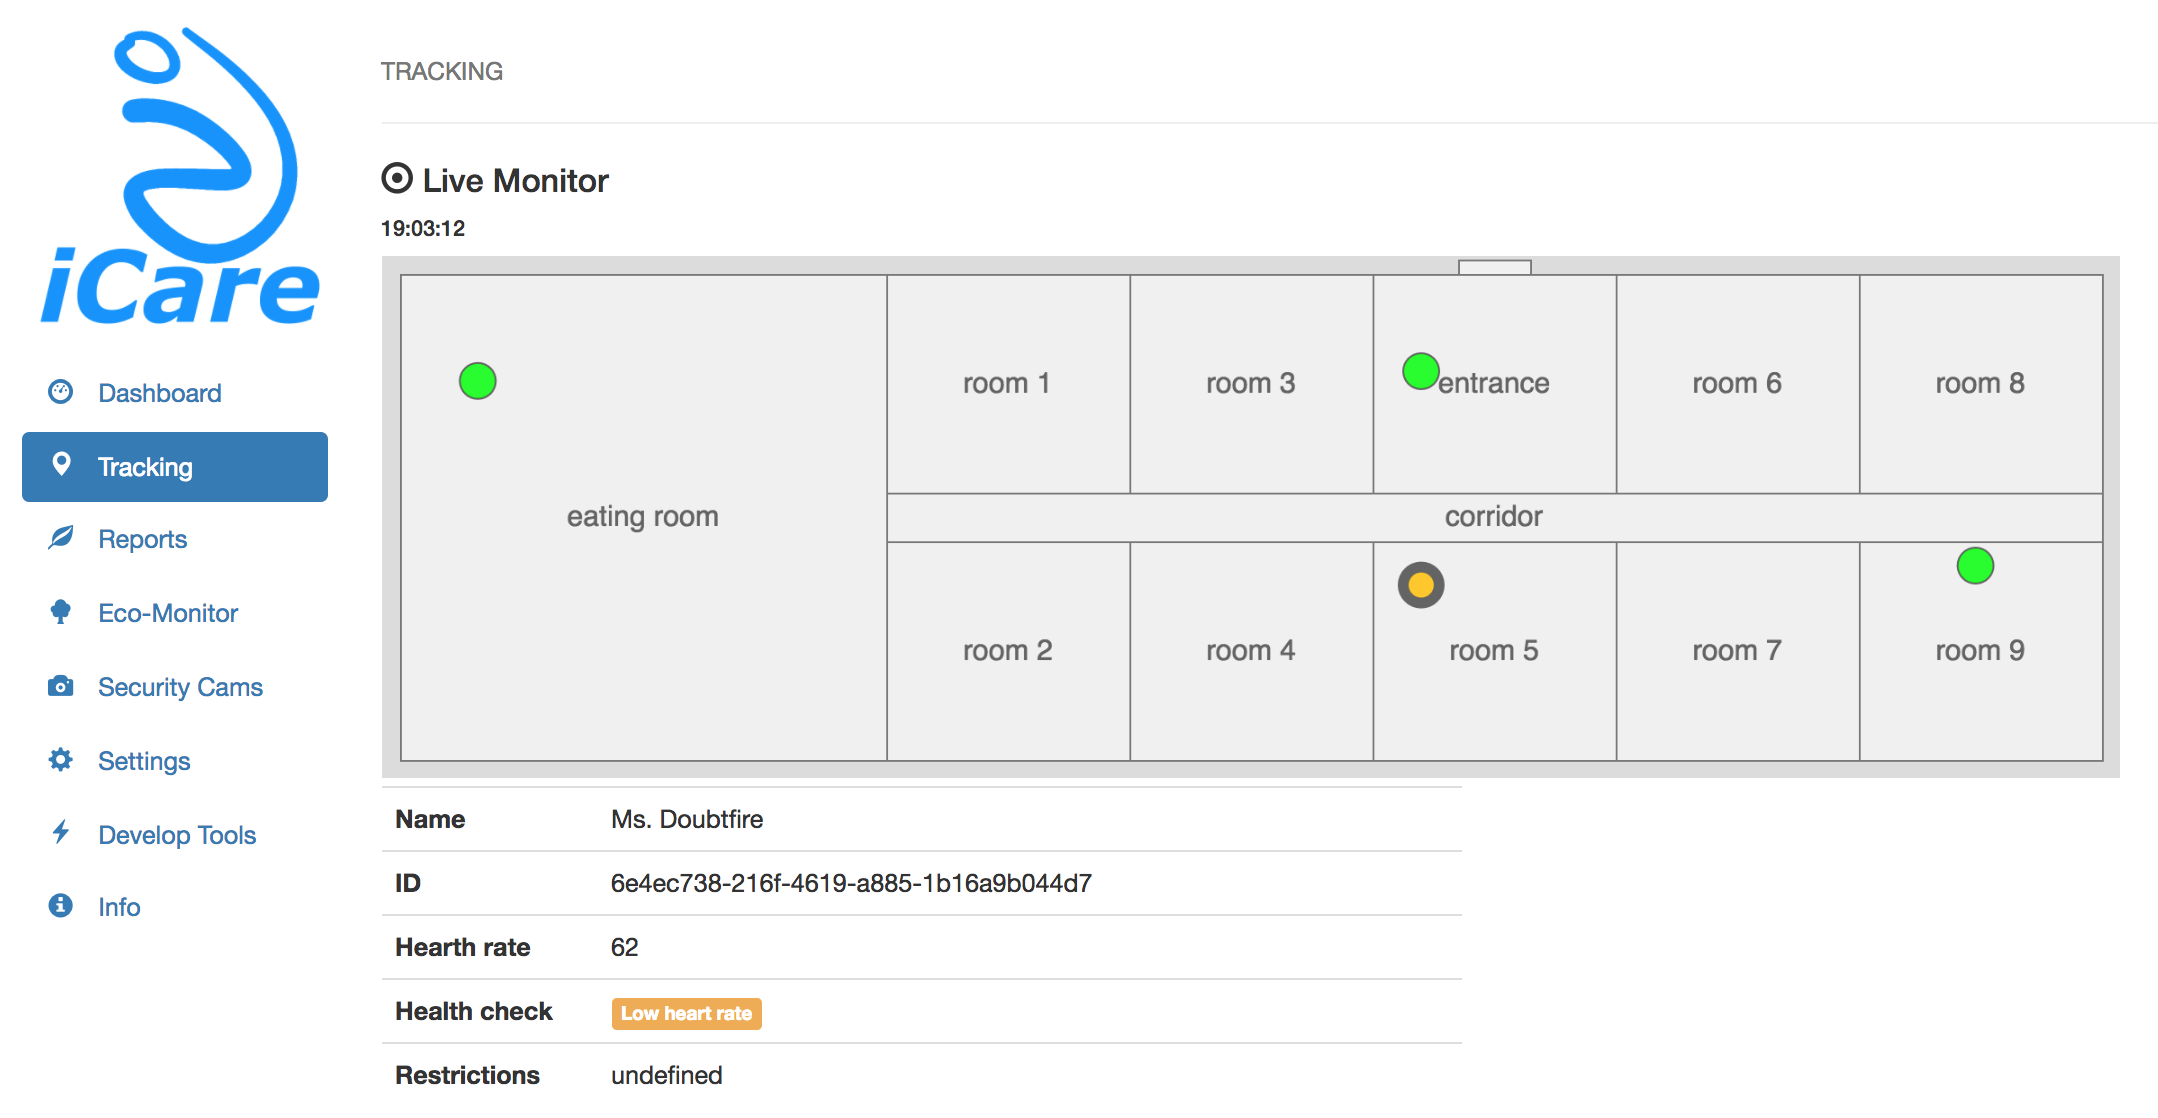
\includegraphics[width =1\textwidth]{images/uiTracking2.png}
	\caption{UI screenshot tracking page}
\end{figure}


\subsection{Eco Monitor}

This page provides an overview of the electricity and water consumption of the last 30 days.
In this case, the data is only loaded once when the web page is loaded, since this data does not change as frequently.

\begin{figure}[H]
	\centering
	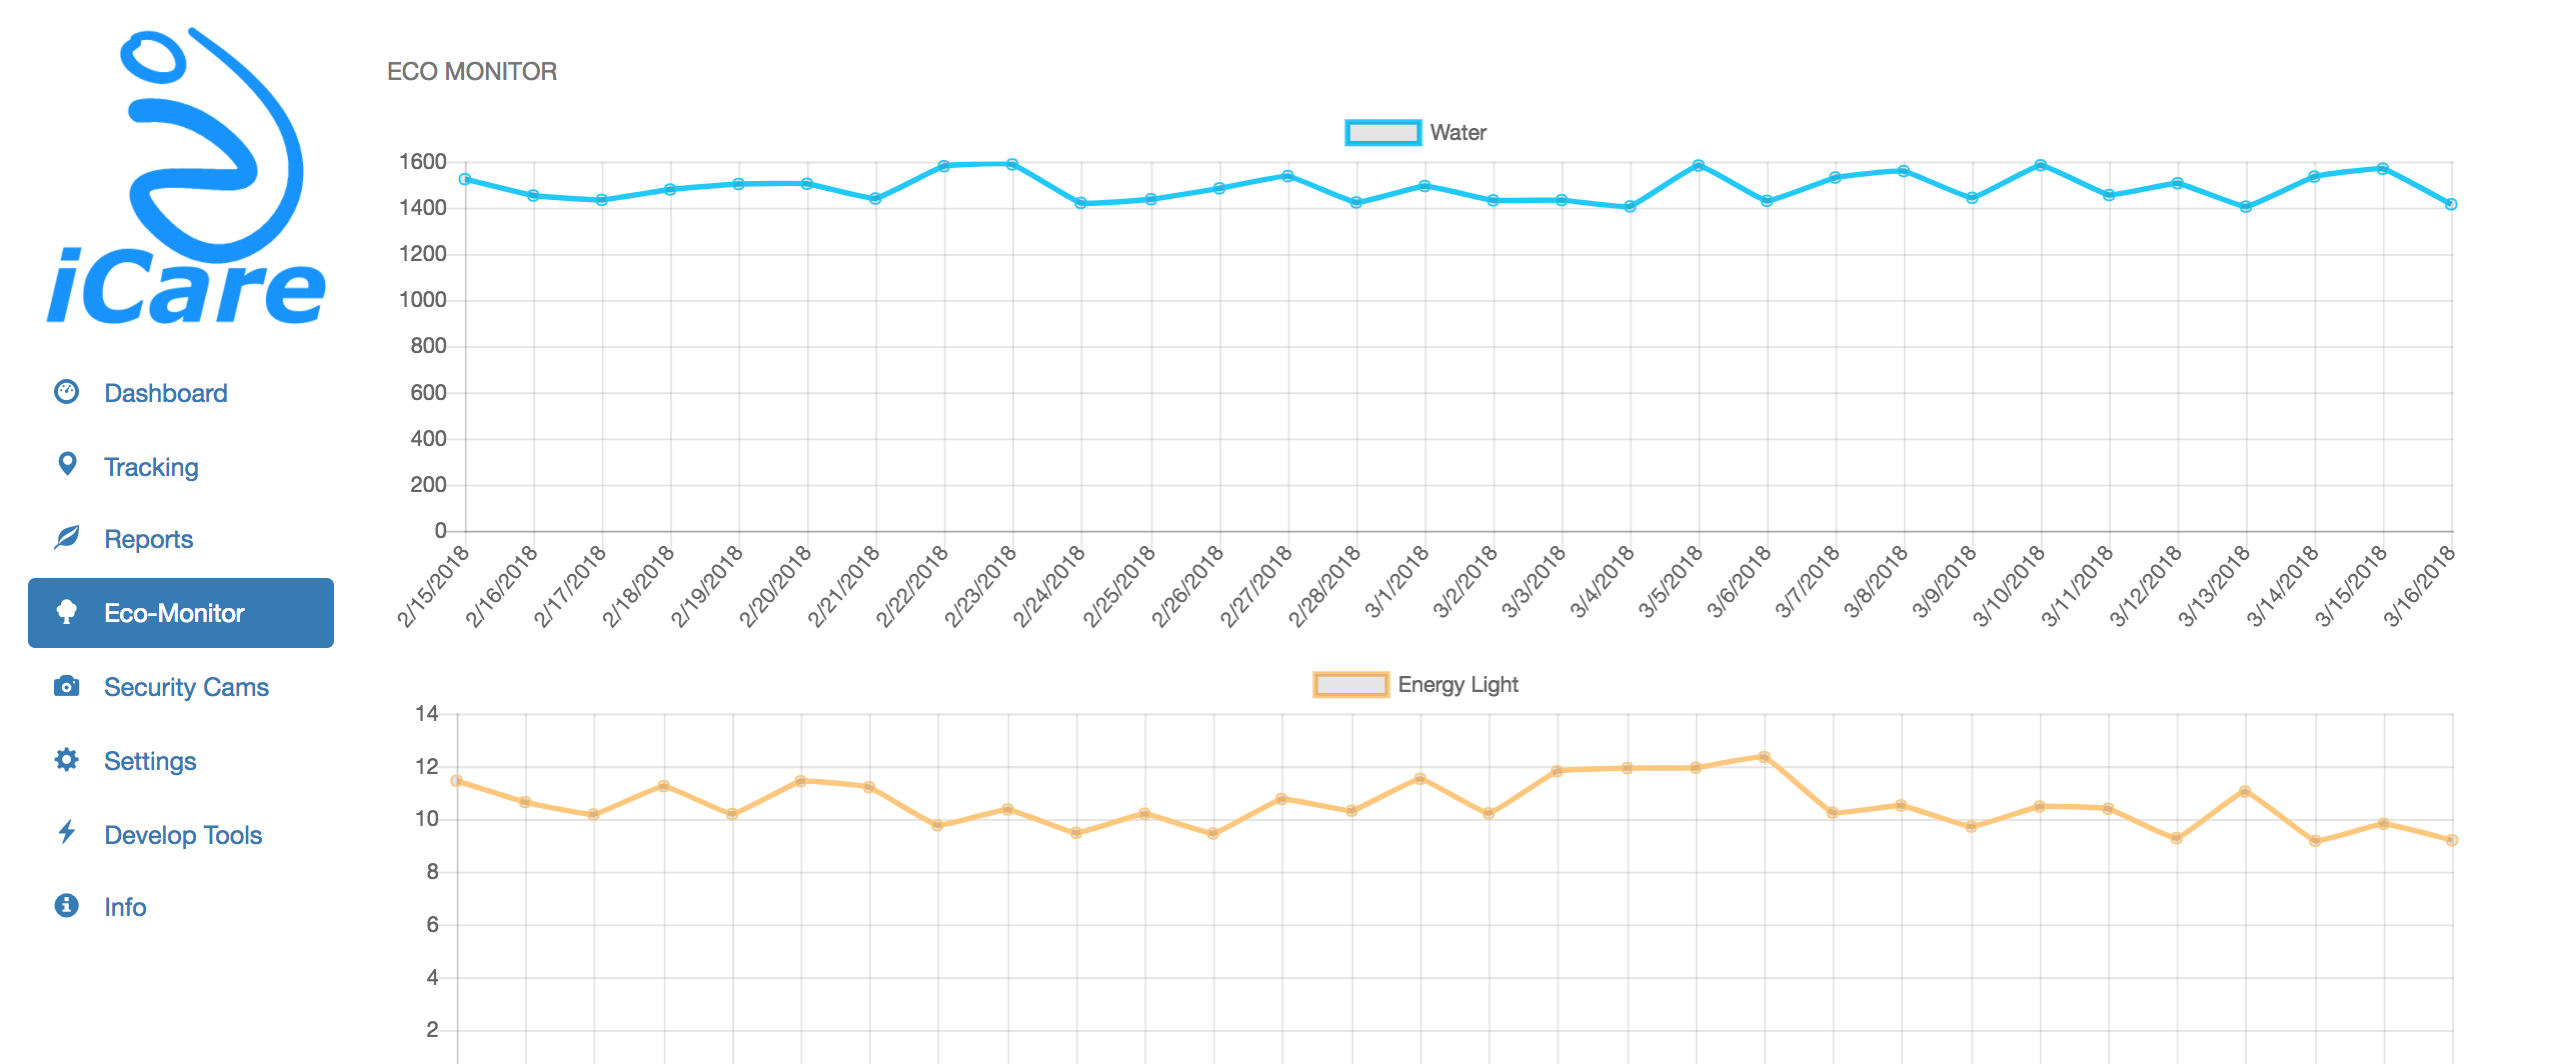
\includegraphics[width =1\textwidth]{images/uiEcoMonitor1.png}
	\caption{UI screenshot Eco Monitor  page}
\end{figure}

\begin{figure}[H]
	\centering
	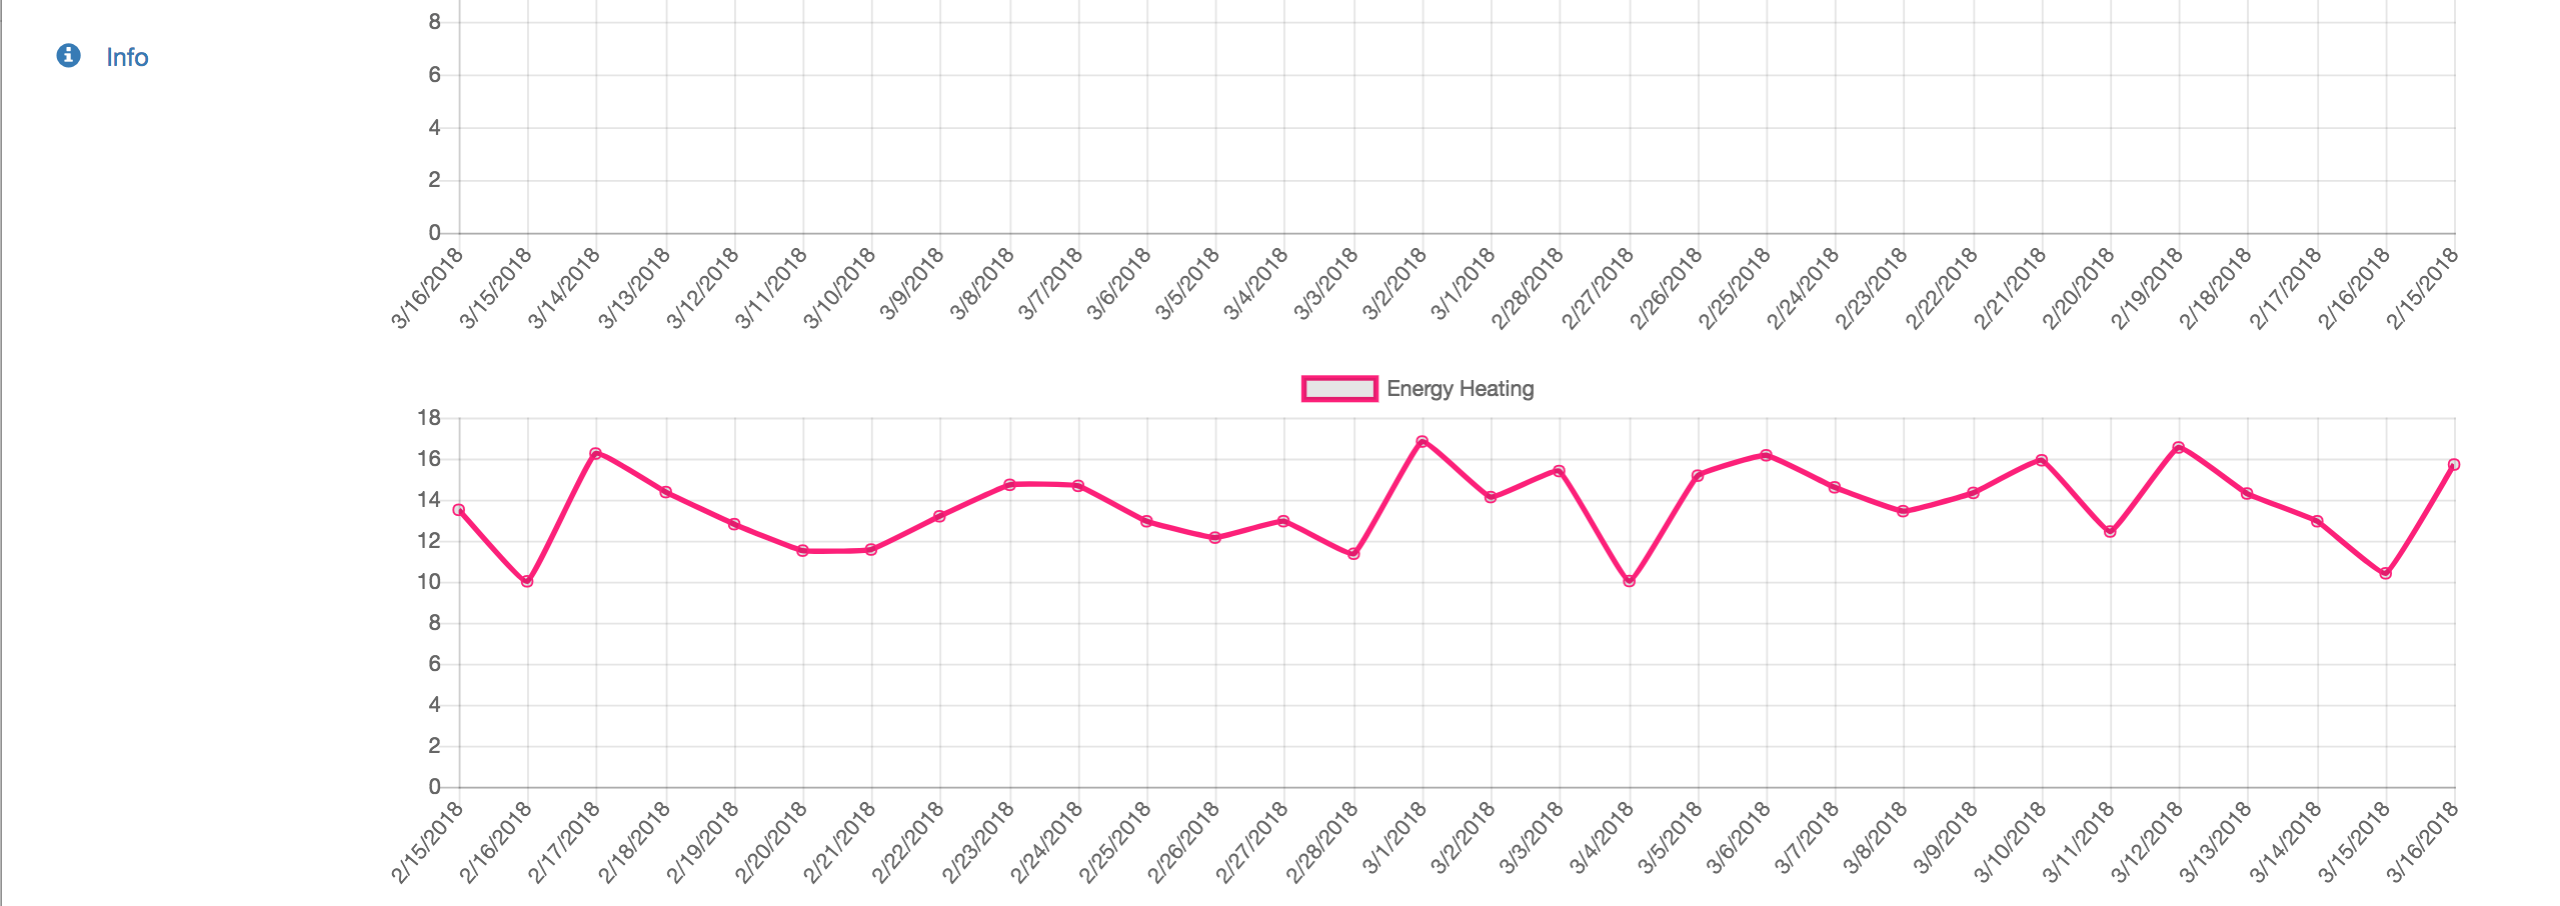
\includegraphics[width =1\textwidth]{images/uiEcoMonitor2.png}
	\caption{UI screenshot Eco Monitor  page}
\end{figure}


\subsection{Camera page}

This page shows the user the last images of the surveillance cameras installed in the Carehome.
At the top he sees the pictures from the reception hall and below the pictures from the outside area. Additionally, a timestamp is diplayed to indicate when the image was taken.
\begin{figure}[H]
	\centering
	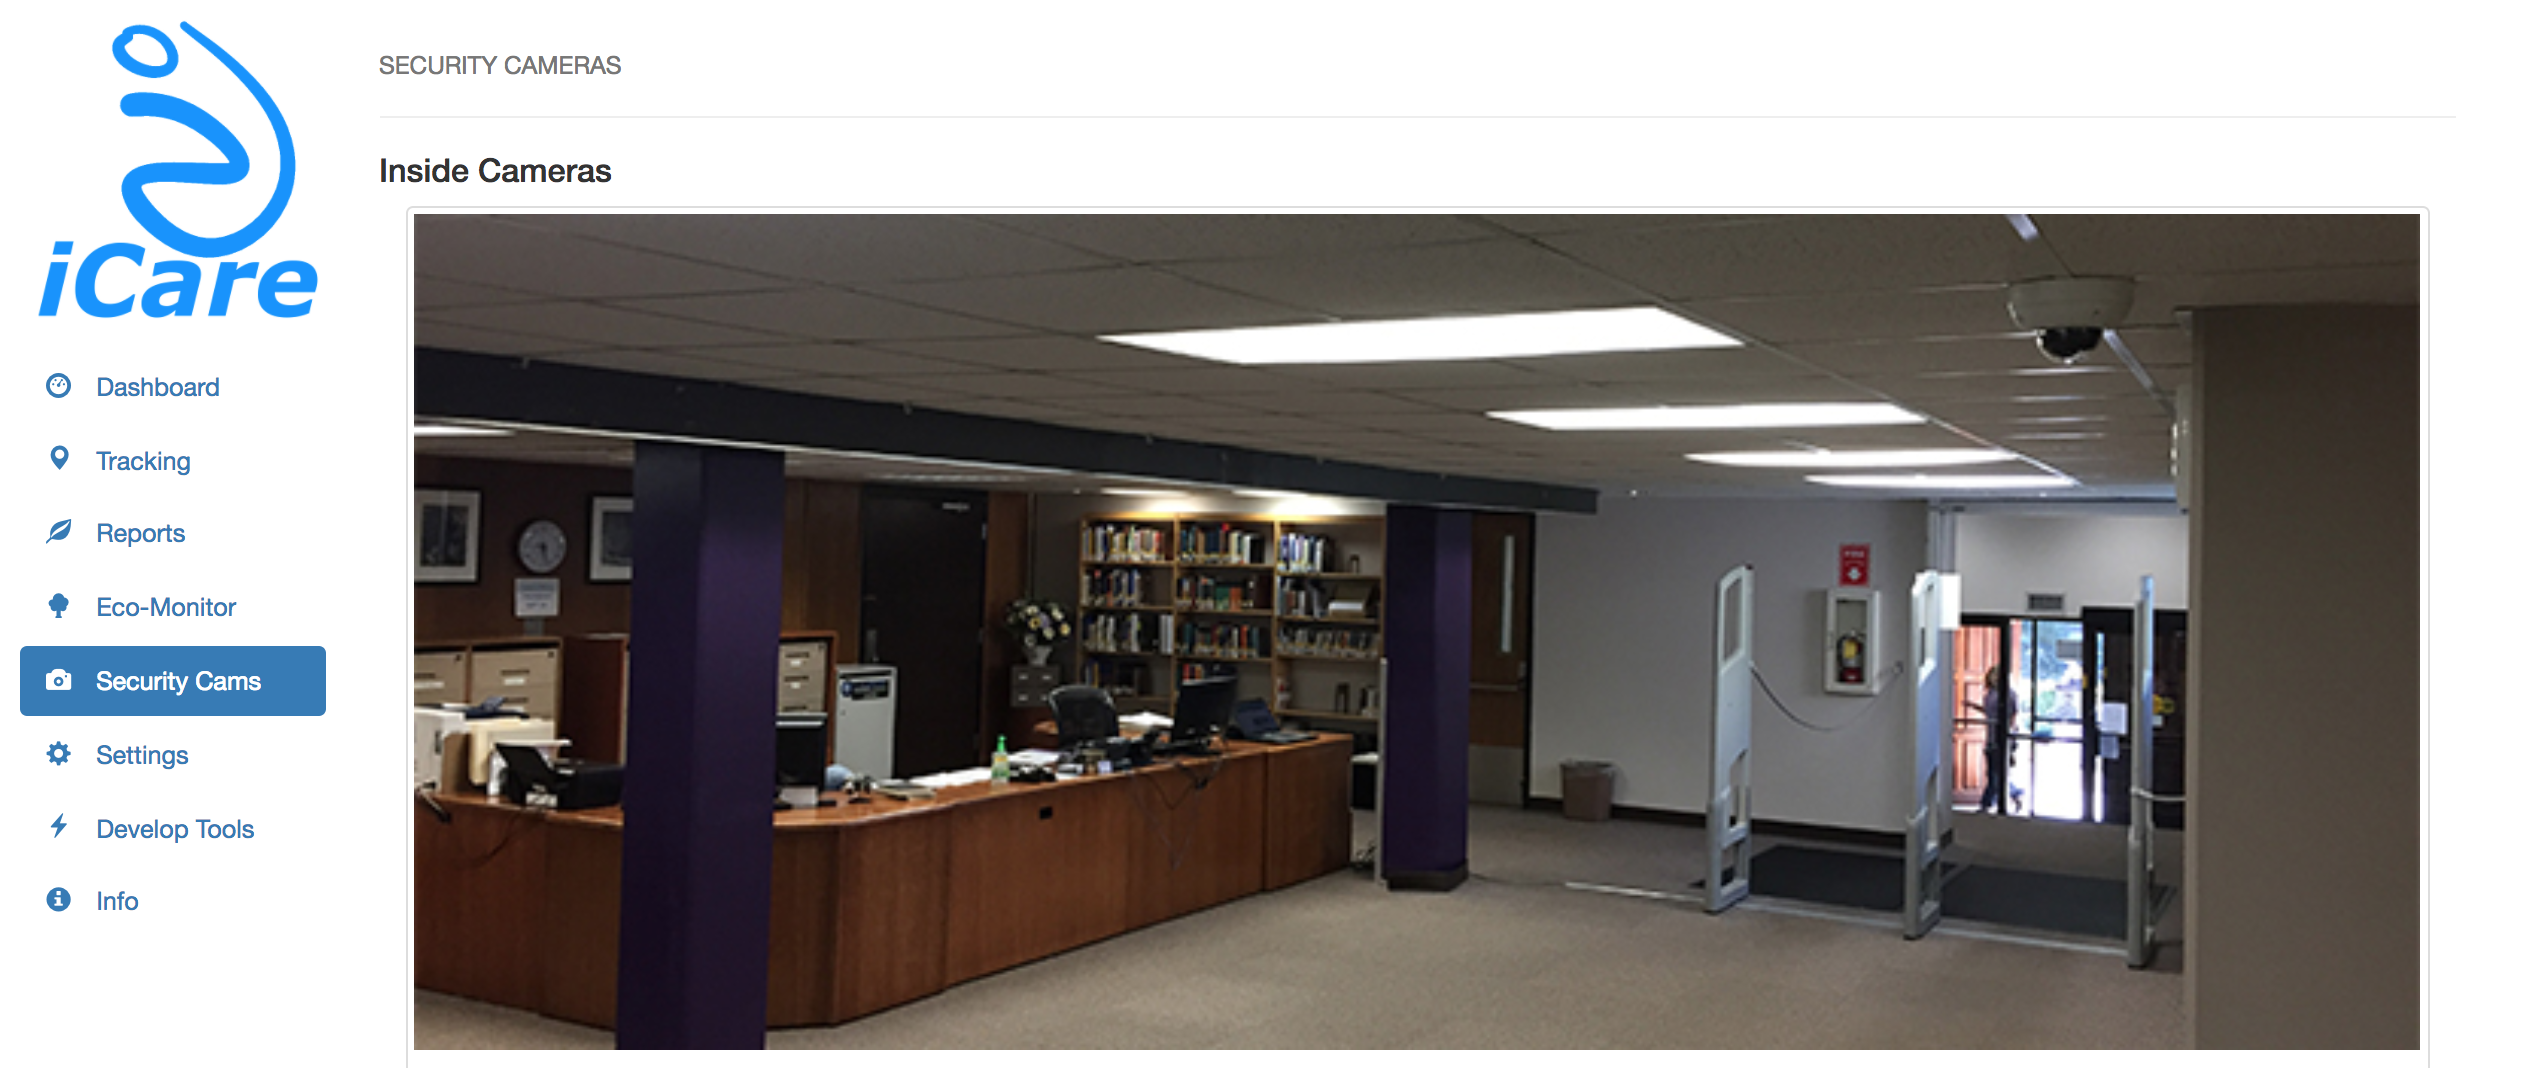
\includegraphics[width =1\textwidth]{images/uiCameras1.png}
	\caption{UI screenshot of cameras page}
\end{figure}

\begin{figure}[H]
	\centering
	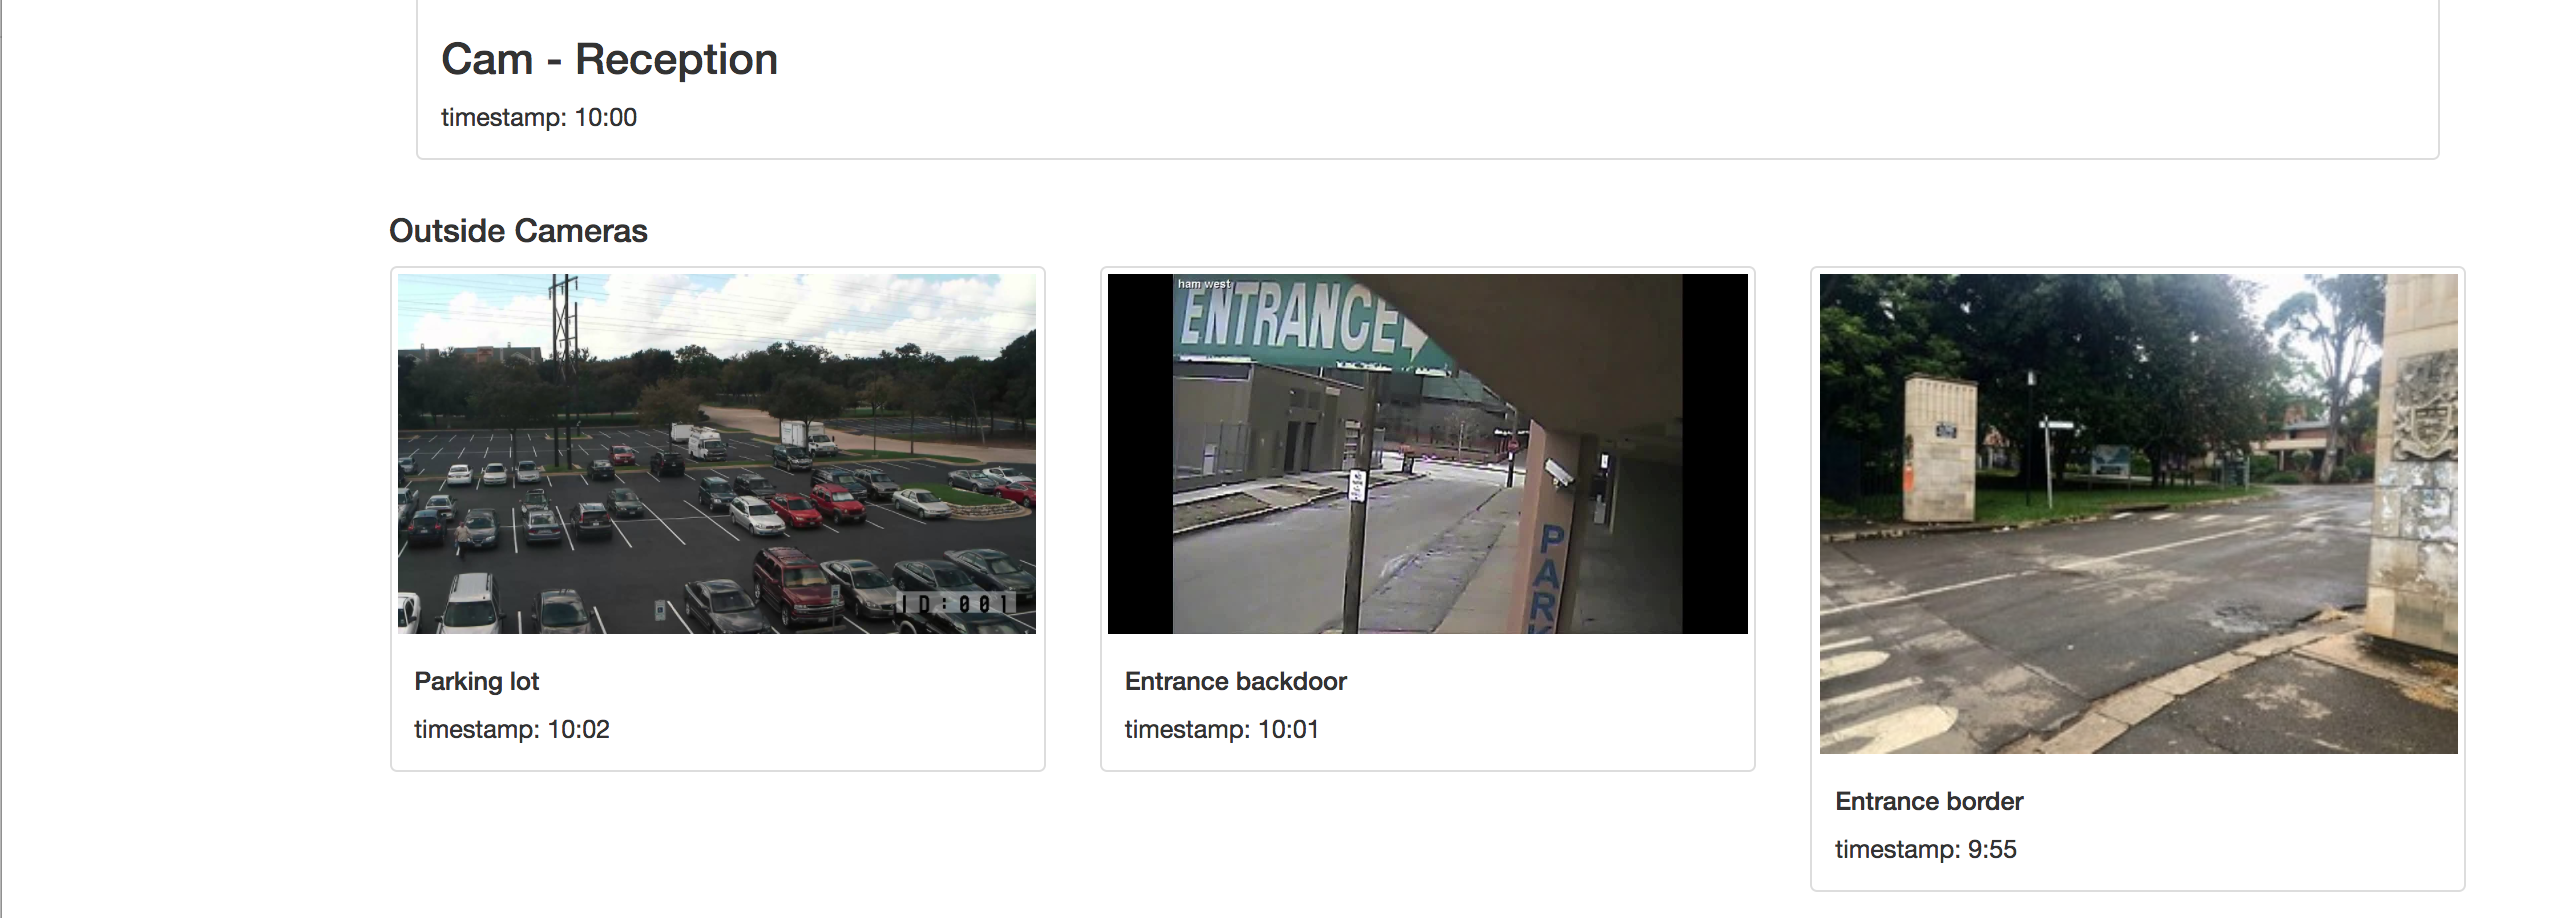
\includegraphics[width =1\textwidth]{images/uiCameras2.png}
	\caption{UI screenshot of cameras page}
\end{figure}

\subsection{Report page}

This page allows you to generate a report for a specified period of time and download it as a pdf file.
The report includes water and electricity consumption. As well as a record of each resident's health check sensors. This feature was not yet implemented completely.


\subsection{Settings page}
This page allows you to configure certain settings on the frontend.
This feature was not yet implemented completely.
